% !TeX program = xelatex
% !TeX encoding = UTF-8
% Layout adapted from billryan/resume (MIT); see TEMPLATE-LICENSE.
\documentclass[10pt,a4paper]{article}
\usepackage[top=1.05cm,bottom=1.05cm,left=1.40cm,right=1.40cm,nohead]{geometry}
\usepackage{fontspec}
\usepackage{graphicx}
\usepackage{enumitem}
\usepackage{titlesec}
\usepackage{fontawesome}
\usepackage[hidelinks]{hyperref}
\usepackage{atbegshi}
\pagestyle{empty}
\setlength{\parindent}{0pt}
\setlength{\parskip}{0pt}
\setlength{\emergencystretch}{2em}
\setmainfont{texgyretermes-regular.otf}[BoldFont=texgyretermes-bold.otf,ItalicFont=texgyretermes-italic.otf]
\setsansfont{texgyreheros-regular.otf}[BoldFont=texgyreheros-bold.otf]
\titleformat{\section}{\large\scshape\raggedright\bfseries}{}{0em}{}[\titlerule]
\titlespacing*{\section}{0pt}{5pt}{3pt}
\titleformat{\subsection}{\normalsize\raggedright}{}{0em}{}
\titlespacing*{\subsection}{0pt}{3pt}{1pt}
\newcommand{\datedsubsection}[2]{\subsection{\textbf{#1}\hfill\normalfont\small #2}}
\newcommand{\name}[1]{\centerline{\fontsize{23}{27}\selectfont\bfseries #1}\vspace{6pt}}
\newcommand{\email}[1]{\faEnvelope\ \href{mailto:#1}{#1}}
\newcommand{\phone}[1]{\faPhone\ #1}
\newcommand{\basicInfo}[1]{\centerline{\sffamily\fontsize{10.5}{13}\selectfont #1}}
\newcommand{\tech}[1]{{\fontsize{9.3}{12}\selectfont\itshape #1\par}\vspace{1pt}}
\setlist[itemize]{label=\textbullet,leftmargin=1.25em,labelsep=0.45em,
  itemsep=1pt,topsep=2pt,parsep=0pt,partopsep=0pt}
\newcount\cvpages
\AtBeginShipout{\global\advance\cvpages by 1
  \ifnum\cvpages>1\PackageError{cv}{Resume exceeds one page}{Shorten the content or adjust spacing.}\fi}
\begin{document}
\fontsize{10.5}{13.2}\selectfont
% Equal side columns keep the name and contacts centered on the page.
\noindent\begin{minipage}[c]{0.14\textwidth}
  \rule{0pt}{2.20cm}
\end{minipage}%
\begin{minipage}[c]{0.72\textwidth}
  \name{Xintong Li}
  \basicInfo{\phone{+65 8697 4095}\quad\textperiodcentered\quad\email{xintong.li@u.nus.edu}}
\end{minipage}%
\begin{minipage}[c]{0.14\textwidth}
  \raggedleft
  \IfFileExists{assets/resume_photo.png}{%
    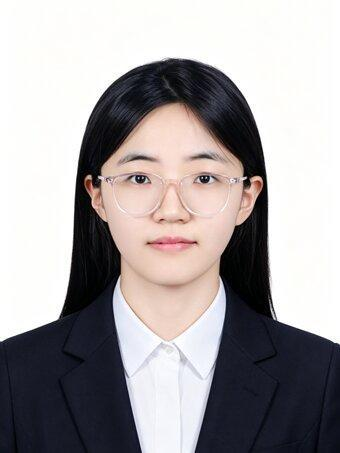
\includegraphics[width=1.65cm]{assets/resume_photo.png}%
  }{\rule{0pt}{2.20cm}}
\end{minipage}\par

\section{\faGraduationCap\ Education}
\datedsubsection{National University of Singapore \quad Master of Computing (MComp)}{Aug 2026 -- Present}
\datedsubsection{Beijing University of Posts and Telecommunications \quad B.Eng. in Communication Engineering}{Sep 2022 -- Jun 2026}
Average score: \textbf{90.47/100}; ranked in the \textbf{top 5\%} of the major. Awarded the \textbf{National Scholarship} and named a \textbf{Beijing Outstanding Graduate}.

\section{\faUsers\ Professional Experience}
\datedsubsection{Kuaishou \quad AI Agent Development Engineer Intern}{May 2026 -- Jul 2026}
\tech{TypeScript / LangGraph / OpenCode / Tool Calling / Multi-Agent / React / Node.js}
Contributed to a multi-agent system comprising \textbf{Code, Design, and Prototype Agents} for UI development, spanning design interpretation, code generation, and interactive prototypes.
\begin{itemize}
  \item \textbf{Structured design context:} Replaced incremental traversal of Figma node trees with parsed, structured context capturing layouts, components, styles, and assets; improved the information supplied to the Code Agent for code generation.
  \item \textbf{Multi-page planning and generation:} Used LangGraph to organize task planning. Persisted page-level context and generated files in a task workspace, generated individual pages in stages, and then added cross-page navigation, interactions, and animations. Used execution results and error messages to drive iterative code fixes.
  \item \textbf{Design-to-code toolchain:} Connected design parsing, context construction, code generation, and project file writing through OpenCode and tool calls. Handled SVG/PNG assets via a CDN, supported RN, KRN, and Vue output, and used the Figma API for Design Agent operations.
  \item \textbf{Generation quality:} Investigated component sizing, missing fonts, and layout discrepancies by comparing generated pages with designs; debugged code and styles and refined the generation workflow.
\end{itemize}

\section{\faCode\ Projects}
\datedsubsection{LLM Agent for Network Fault Root Cause Analysis}{Dec 2025 -- Mar 2026}
\tech{Python / Qwen2.5-7B-Instruct / PEFT / LoRA / GRPO / LangChain / ReAct / RAG}
Built an agent for multi-step diagnosis of network faults from operational data and retrieved knowledge.
\begin{itemize}
  \item \textbf{Training data:} Created \textbf{2,400 SFT examples} from TeleLogs. Generated reasoning traces with exclusion, contradiction, rule-based, and statistical strategies, then used a teacher model to consolidate and standardize correct traces.
  \item \textbf{Model adaptation:} Fine-tuned Qwen2.5-7B-Instruct with PEFT/LoRA and applied GRPO to improve final root-cause selection.
  \item \textbf{Agent diagnosis:} Built ReAct tools for table parsing, fault-interval identification, cell geometry, and neighboring-cell interference analysis; combined them with a rule knowledge base and RAG for multi-step reasoning.
  \item \textbf{Results:} Pass@1 rose from 12.04\% (base model) to 53.59\% (fine-tuned) and \textbf{76.50\%} (with agent); Pass@4 rose from 12.50\% to 54.86\% and \textbf{78.36\%}, respectively.
\end{itemize}
\vspace{3pt}
\datedsubsection{CADDesigner: Agent-Based CAD Model Generation}{Jun 2025 -- Sep 2025}
\tech{Python / LangChain / Claude Sonnet / CadQuery / PythonOCC / ReAct / Function Calling}
Built a text/image-to-CAD workflow for code generation, 3D model construction, rendering, and iterative refinement.
\begin{itemize}
  \item \textbf{Modeling workflow:} Orchestrated requirement parsing, code generation, model construction, three-view rendering, visual assessment, and iterative revision with LangChain and tool calls.
  \item \textbf{Multimodal generation:} Used Claude Sonnet to extract geometric features, structural relationships, and constraints from text and reference images, then generate parametric CadQuery/PythonOCC code.
  \item \textbf{Visual feedback:} Executed code in a sandbox, rendered standard three-view drawings, and fed the results back to the agent to revise or regenerate code when the model differed from the requirements.
  \item \textbf{Results:} On CAD-VGDrawing, achieved IoU 0.2769, CD 0.1097, HD 0.4347, and 100.0\% valid-model generation success (SUC).
\end{itemize}

\section{\faCogs\ Skills}
\textbf{Development:} Linux, Shell, Git, Conda, remote GPU servers; familiar with Unity.\par
\textbf{Model training:} LoRA/QLoRA, PEFT, GRPO; dataset construction, domain adaptation, and evaluation.\par
\textbf{Agents:} LangGraph, LangChain, ReAct, tool calling, multi-agent systems, RAG.
\end{document}
